\clearpage
\setcounter{page}{1}
\maketitlesupplementary
\appendix
\section{Idealized Analysis: Statements and Proofs}\label{app:theory}
Let $\bm{x}=(x_0,\dots,x_{N-1})$ be one channel of a patch, $f_k=kf_s/N$, and consider
$1\le k\le K=\lfloor(N-1)/2\rfloor$. Define $X_k=\sum_t x_te^{-i2\pi kt/N}$,
$I_k=|X_k|^2/N$, $\varphi_k=\arg X_k$.

\begin{assumption}[stationary Gaussian; state acts through the spectrum]\label{as:gauss}
Given the state $\theta$, $\bm{x}$ is a segment of a zero-mean weakly stationary Gaussian
process with positive spectral density $S_\theta$, continuous except at finitely many points
and continuous at the $f_k$ used.
\end{assumption}

\begin{lemma}[Brillinger 1981, Thm.~4.4.1]\label{lem:dft}
Under Assumption~\ref{as:gauss}, as $N\to\infty$, for a fixed set of frequencies,
$X_k/\sqrt{NS_\theta(f_k)}$ converges in distribution to independent standard circular complex
Gaussians. Hence approximately $I_k\approx S_\theta(f_k)E_k$ with $E_k$ i.i.d.\
$\mathrm{Exp}(1)$, and $\varphi_k$ i.i.d.\ uniform on $[0,2\pi)$, independent of $\{I_k\}$,
with a distribution that does not depend on $\theta$.
\end{lemma}
\noindent The Whittle approximation \cite{whittle1953} follows:
\begin{equation}\label{eq:whittle}
-\log p(\bm{x}\mid\theta)\approx\sum_{k=1}^{K}\Bigl[\log S_\theta(f_k)+\frac{I_k}{S_\theta(f_k)}\Bigr]+\text{const}.
\end{equation}

\begin{proposition}[phase is ancillary]\label{prop:suff}
In the Whittle model of \eqref{eq:whittle}, $(I_1,\dots,I_K)$ is sufficient for
$\theta$, and the distribution of $(\varphi_1,\dots,\varphi_K)$ does not depend on $\theta$.
\end{proposition}
\begin{proof}
The data enter \eqref{eq:whittle} only through $\{I_k\}$ (Fisher--Neyman factorization); the
phase distribution is given by Lemma~\ref{lem:dft}.
\end{proof}
\noindent This is a statement about a patch's marginal spectral likelihood. It does not
imply that its phase is independent of visible context. Both the magnitude and phase of a
Fourier coefficient fluctuate conditional on the state; correlations with neighbouring
samples or other channels can make part of that realization predictable.

\begin{assumption}[approximately flat bands; in-band observation]\label{as:band}
Let $\mathcal{F}=[0.5,45]$\,Hz contain disjoint bands $B_1,\dots,B_5$, possibly separated by
transition regions. (i) For $f_k\in B_b$, $S_\theta(f_k)\approx s_b(\theta)$. (ii) The
observation consists only of the in-band coefficients $\{X_k:f_k\in\bigcup_bB_b\}$
(equivalently, the signal is first band-passed to $\bigcup_bB_b$). Let
$m_b=\#\{k:f_k\in B_b\}$.
\end{assumption}
\noindent Part (ii) avoids any conflict with the continuity in Assumption~\ref{as:gauss}: the
spectrum may vary continuously everywhere; (i) only requires it to be nearly constant within
each band.

\begin{proposition}[band power in the restricted Whittle model]\label{prop:mle}
Under Assumption~\ref{as:band} with equality in (i), in the Whittle model of \eqref{eq:whittle},
$P_b=m_b^{-1}\sum_{f_k\in B_b}I_k$ is sufficient for $\bm{s}=(s_b)_b$, $\hat s_b=P_b$ is the
maximum-likelihood estimate, and $\log P_b$ is the MLE of $\log s_b$.
\end{proposition}
\begin{proof}
By (ii) the likelihood involves only in-band bins; by (i),
$-\log p(\bm{x}\mid\bm{s})\approx\sum_b[m_b\log s_b+m_bP_b/s_b]+\text{const}$. The data enter
only through $P_b$; setting the derivative in $s_b$ to zero gives $\hat s_b=P_b$.
\end{proof}
\begin{remark}
Prop.~\ref{prop:mle} is exact within this restricted likelihood; it is an idealization for
non-flat spectra and finite EEG patches. It does not establish sufficiency for spectral
information outside the observed bands or for arbitrary downstream labels. For an
ideal circular band-pass $\tilde h_b$, Parseval gives
$\frac1N\sum_t((\tilde h_b*\bm{x})_t)^2=\frac{2m_b}{N}P_b$, a per-band constant factor. The
main target (Eq.~\eqref{eq:target}, with $N{=}P$) uses
$\log(a_bP_b+\varepsilon)$, where $a_b=2m_b/N$. At zero floor this is $\log P_b+\log a_b$.
At positive floor the transformation remains invertible, but its noise distribution is no
longer a constant shift of the zero-floor log distribution.
\end{remark}

\begin{proposition}[conditional noise of zero-floor log power]\label{prop:var}
In the independent-bin Whittle model with exactly flat bands,
$P_b=s_b(\theta)G_b$ conditional on $\theta$, where
$G_b\sim\mathrm{Gamma}(m_b,1/m_b)$ (shape, scale). Thus
\begin{align*}
\Var[P_b\mid\theta]&=s_b(\theta)^2/m_b,\\
\E[\log P_b\mid\theta]&=\log s_b(\theta)+\psi(m_b)-\log m_b,\\
\Var[\log P_b\mid\theta]&=\psi'(m_b)\approx1/m_b.
\end{align*}
\end{proposition}
\begin{proof}
A sum of $m$ i.i.d.\ $\mathrm{Exp}(1)$ is $\mathrm{Gamma}(m,1)$, whose logarithm has mean
$\psi(m)$ and variance $\psi'(m)$.
\end{proof}
\noindent For Eq.~\eqref{eq:target}, the additional term
$\log(G_b+\varepsilon/[a_bs_b(\theta)])$ generally has a state-dependent mean and variance.
The zero-floor identities are therefore reference calculations, not exact noise identities
for the implemented target; no negligible-floor approximation is assumed for all observations.

\begin{assumption}[shared state and independent-patch idealization]\label{as:persist}
The context $\bm{c}$ and the masked patch share the state $\theta$, and given $\theta$ the
target of the masked patch is independent of $\bm{c}$.
\end{assumption}
\noindent This is an additional idealization used below for band power, not a consequence of
phase ancillarity or patch-local target computation. Adjacent patches and other channels may
remain correlated conditional on the state. The correlated waveform model below does not
impose this independence assumption.

\begin{proposition}[risk decomposition for any target]\label{prop:decomp}
For a square-integrable target $Y$, let $g(\bm{c})=\E[Y\mid\bm{c}]$ and
$V(\bm{c})=\operatorname{Cov}(Y\mid\bm{c})$. Under squared Euclidean loss,
\begin{align*}
R(f)&=\E\|f(\bm{c})-Y\|^2,\\
R^*&=\inf_f R(f)=\E\operatorname{tr}V(\bm{c}),\\
R(f)-R^*&=\E\|f(\bm{c})-g(\bm{c})\|^2.
\end{align*}
For scalar $Y$ under Assumption~\ref{as:persist}, writing
$\mu(\theta)=\E[Y\mid\theta]$ and $\sigma^2(\theta)=\Var(Y\mid\theta)$ gives
$R^*=\E[\Var(\mu(\theta)\mid\bm{c})]+\E[\sigma^2(\theta)]$.
\end{proposition}
\begin{proof}
Expanding $f-Y=(f-g)+(g-Y)$, the cross term vanishes after conditioning on $\bm{c}$.
The last identity follows from conditional independence:
$\E[Y\mid\bm{c}]=\E[\mu(\theta)\mid\bm{c}]$ and
$\Var(Y\mid\bm{c})=\Var(\mu(\theta)\mid\bm{c})+\E[\sigma^2(\theta)\mid\bm{c}]$; take
expectations over $\bm{c}$.
\end{proof}
\noindent For zero-floor $Y_b=\log P_b$ under Assumption~\ref{as:persist} and the exact
flat-band Whittle model, let $k_b=\psi(m_b)-\log m_b$. Then
\begin{align*}
g_b(\bm{c})&=\E[\log s_b(\theta)\mid\bm{c}]+k_b,\\
V_b(\bm{c})&=\psi'(m_b)+\Var(\log s_b(\theta)\mid\bm{c}).
\end{align*}
Both terms in the Bayes risk are irreducible for a fixed observed context. Only excess
prediction error above this risk is reducible by improving $f$. Predicting a posterior average
of spectral levels need not identify $\theta$ or a downstream label.

\noindent\emph{A separate correlated waveform model.} Applying the independence assumption
to a zero-mean waveform would give $g(\bm{c})=\bm{0}$. Instead, for a fixed mask suppose
$(\bm{x}_M,\bm{c})$ is jointly zero-mean Gaussian conditional on $\theta$, allowing nonzero
cross-covariance. Its conditional mean and innovation covariance are
\begin{align*}
\bm{m}_\theta(\bm{c})&=\Sigma_{Mc,\theta}\Sigma_{cc,\theta}^{-1}\bm{c},\\
Q_\theta&=\Sigma_{MM,\theta}
-\Sigma_{Mc,\theta}\Sigma_{cc,\theta}^{-1}\Sigma_{cM,\theta},
\end{align*}
assuming $\Sigma_{cc,\theta}$ is invertible. With the state unknown, total expectation and
covariance give
\begin{align*}
g_{\mathrm{raw}}(\bm{c})&=\E[\bm{m}_\theta(\bm{c})\mid\bm{c}],\\
V_{\mathrm{raw}}(\bm{c})&=\E[Q_\theta\mid\bm{c}]
+\operatorname{Cov}(\bm{m}_\theta(\bm{c})\mid\bm{c}).
\end{align*}
Thus the known-state innovation alone omits posterior state uncertainty. For per-coordinate
waveform MSE, the Bayes risk is $\E\operatorname{tr}V_{\mathrm{raw}}(\bm{c})/|M|$.

\begin{proposition}[the irreducible part adds gradient noise, not signal]\label{prop:grad}
Let $Y=g(\bm{c})+\xi$ with $g(\bm{c})=\E[Y\mid\bm{c}]$, $\E[\xi\mid\bm{c}]=0$ and
$\mathrm{Cov}(\xi\mid\bm{c})=\Sigma(\bm{c})$. For a model $f_w$ with Jacobian
$J=\partial f_w(\bm{c})/\partial w$ and loss $\ell=\tfrac12\|f_w(\bm{c})-Y\|^2$, the stochastic
gradient $G=J^\top(f_w(\bm{c})-Y)$ satisfies
$\E[G]=\nabla_w\tfrac12\E\|f_w(\bm{c})-g(\bm{c})\|^2$ and
$\mathrm{Cov}(G)=\mathrm{Cov}\bigl(J^\top(f_w-g)\bigr)+\E\bigl[J^\top\Sigma(\bm{c})J\bigr]$.
\end{proposition}
\begin{proof}
$G=J^\top(f_w-g)-J^\top\xi$. Conditioning on $\bm{c}$, $\E[J^\top\xi\mid\bm{c}]=0$, so the
second term has mean zero and is uncorrelated with the first; its covariance is
$\E[J^\top\E[\xi\xi^\top\mid\bm{c}]J]$.
\end{proof}
\noindent The expected gradient depends only on the excess prediction error $f_w-g$; the
conditional residual contributes $\E[J^\top\Sigma J]$. Here $\Sigma(\bm{c})=V(\bm{c})$ is
the \emph{full} conditional covariance. For the vector of zero-floor log band powers under
the independent-patch, flat-band Whittle model, let
$\bm{\lambda}(\theta)=(\log s_b(\theta))_{b=1}^5$. Then
\[
\Sigma_{\mathrm{BP}}(\bm{c})=\operatorname{diag}_{b}\{\psi'(m_b)\}
+\operatorname{Cov}(\bm{\lambda}(\theta)\mid\bm{c}).
\]
For the correlated waveform model it is $V_{\mathrm{raw}}(\bm{c})$ above. The positive floor
changes the band-power noise identities, and neither target's gradient covariance is determined
by its marginal target variance alone.

For an $L$-smooth, lower-bounded population risk $\mathcal{R}(w)$, unbiased stochastic gradients
with variance bounded by $\sigma_G^2$, independent mini-batch samples of size $B$, and suitable
step sizes, a standard upper bound for returning an iterate with
$\E\|\nabla_w\mathcal{R}\|^2\le\epsilon$ has order
$L\Delta/\epsilon+L\Delta\sigma_G^2/(B\epsilon^2)$, where $\Delta$ is the initial risk gap
\cite{ghadimi2013}. This upper bound can worsen with gradient variance; it does not establish
that one target necessarily needs proportionally more steps, or bound steps to a downstream
score. Comparing the targets also changes $g$, $J$, loss scale and smoothness. The gradient
identity therefore motivates a possible mechanism rather than proving the observed speedup.

\noindent\emph{Empirical comparison.} On TUAB evaluation windows (Table~\ref{tab:target_r2}) the
band-power model's error at epoch 16 is $0.16/0.12/0.10/0.06/0.08$ for
$\delta/\theta/\alpha/\beta/\gamma$, against an idealized noise $\psi'(m_b)$ of
$0.40/0.40/0.28/0.08/0.09$ (Table~\ref{tab:bins}). Errors below these reference values show
that the idealized calculation is not a quantitative noise floor for this setting. Contextual
dependence, non-flat spectra, finite patches and the positive floor can all affect the
comparison; these measurements do not isolate a cause or establish a general bound on Bayes
risk. The waveform model explains $3\%$ of its target's variance. Achieved $R^2$ measures the
trained predictor, not the maximum predictability of either target.

\begin{table}[h]\centering\small
\caption{Ideal rectangular bands at our patch length ($N{=}200$, $f_s{=}256$\,Hz,
$\Delta f{=}1.28$\,Hz): number of Fourier bins and idealized conditional sampling noise of
zero-floor $\log P_b$ (Prop.~\ref{prop:var}). These are the bands and bin counts of the main
target; the noise values are not measured conditional variances for Eq.~\eqref{eq:target}.}
\label{tab:bins}
\setlength{\tabcolsep}{4pt}
\begin{tabular}{l c c c}
\toprule
Band & Range (Hz) & $m_b$ & $\mathrm{sd}[\log P_b\mid\theta]=\sqrt{\psi'(m_b)}$\\
\midrule
$\delta$ & 0.5--4 & 3 & 0.63\\
$\theta$ & 4--8 & 3 & 0.63\\
$\alpha$ & 8--13 & 4 & 0.53\\
$\beta$ & 13--30 & 13 & 0.28\\
$\gamma$ & 30--45 & 12 & 0.29\\
\bottomrule
\end{tabular}
\end{table}

\section{Downstream Data Details}\label{app:data}
\noindent\textbf{Beyond-sleep tasks.} For MA, Mumtaz and PhysioNet-MI we reproduce CBraMod's
\texttt{preprocessing\_*.py} scripts line by line (file ordering, split slices, channel
selection, filtering, resampling to 200\,Hz and window length) and store the samples once;
every model is probed on these samples. FACED's official processed release was not
reachable from our region; we rebuilt it from the public raw BIDS recordings following the
FACED paper (last 30\,s of each clip, 0.05--47\,Hz, common average reference, 250\,Hz,
bad-channel interpolation; no ICA) and then applied CBraMod's FACED preprocessing. Our input
convention adds, for our model only, 0.5--45\,Hz band-pass, resampling to 256\,Hz and
per-recording robust scaling of the same samples, restricted to the 19 standard leads, which
all four tasks contain.

% auto-generated by make_arxiv_tables.py -- do not edit
% Detailed per-dataset results (REVE-style). Counts filled in from dataset_counts.json.
\section{Detailed Results per Dataset}\label{app:fullmetrics}
Table~\ref{tab:overview} reports balanced accuracy only. Here every dataset is described and
given its own table with the metrics that prior EEG foundation models report: balanced accuracy,
Cohen's $\kappa$ and weighted F1 for every task, and additionally AUROC and AUC-PR for the binary
tasks. All numbers come from the strict linear probe of Sec.~\ref{sec:lpproto}, measured by us
with the released weights on identical samples and splits; balanced accuracy on the validation
split is the only selection criterion (the regularization $C$ and, for REVE, the readout).

\noindent\textbf{Uncertainty.} The external models are released as single checkpoints, so we
evaluate one checkpoint of SpecBraM as well, our main released model, and quantify the
uncertainty of every model in the same way. For mixed-label or multiclass tasks we use ordinary
cluster resampling of test subjects with replacement. For binary tasks whose subjects each
have one true label, subjects are resampled within true-label strata. For TUEV the cluster unit
is the recording, since its evaluation files are anonymized. Candidate resamples missing any
test-set class are discarded until 1{,}000 valid replicates are obtained. Every metric is
recomputed on the pooled samples of the drawn clusters; the 2.5th and 97.5th percentiles form
the nominal 95\% confidence interval. These intervals describe test-cohort sampling variation
conditional on the fitted checkpoint and probe, not pretraining-seed variability. To show the variation of our
pretraining, each table also lists SpecBraM's mean and standard deviation over its three
pretraining seeds; this row is not used for the comparison.

\noindent\textbf{Confusion matrices.} For every dataset we also show the row-normalized confusion
matrices of SpecBraM and of REVE, the strongest baseline, and their difference, to see which
classes each model recognizes.

\noindent\textbf{Paired differences.} Overlapping intervals do not imply that two models are
equivalent, so we also bootstrap the difference itself: on each of the 1{,}000 resamples the
score of every external model is subtracted from SpecBraM's on the same drawn clusters,
preserving the pairing (Table~\ref{tab:paired}). The generated table gives the nominal,
unadjusted 95\% intervals for each difference; no correction for multiple comparisons is
applied. An interval excluding zero is evidence of a difference under this procedure. An
interval containing zero indicates no detected difference, not equivalence or noninferiority.
The intervals condition on the evaluated checkpoints and do not include training variability.
% auto-generated by make_arxiv_tables.py -- do not edit
\begin{table*}[t]\centering\small
\setlength{\tabcolsep}{6pt}
\caption{\textbf{Paired bootstrap of the difference} in balanced accuracy (points) between
SpecBraM's main checkpoint and each external model, computed on the same 1{,}000 resamples of
the test subjects (TUEV: recordings), with its nominal, unadjusted 95\% confidence interval.
Positive: SpecBraM better. Bold: the interval excludes zero; this is not an equivalence test.}
\label{tab:paired}
\begin{tabular}{l ccccc}
\toprule
Dataset & CBraMod & LaBraM-Base & BIOT & CSBrain & REVE-Base\\
\midrule
ISRUC & \ci{\textbf{+6.2}}{+4.28}{+8.01} & \ci{\textbf{+3.8}}{+1.93}{+5.41} & \ci{\textbf{+5.4}}{+2.81}{+8.11} & \ci{\textbf{+6.0}}{+4.85}{+7.11} & \ci{-0.3}{-1.89}{+1.36} \\
HMC & \ci{\textbf{+12.3}}{+9.53}{+15.51} & \ci{\textbf{+11.0}}{+8.45}{+13.63} & \ci{\textbf{+8.4}}{+6.06}{+10.89} & \ci{\textbf{+13.1}}{+9.82}{+16.35} & \ci{\textbf{+3.8}}{+1.83}{+5.90} \\
TUAB & \ci{\textbf{+3.5}}{+1.09}{+6.12} & \ci{\textbf{+3.7}}{+1.52}{+6.06} & -- & \ci{\textbf{+4.1}}{+1.63}{+6.44} & \ci{-0.8}{-2.71}{+1.21} \\
TUEV & \ci{+3.0}{-3.06}{+9.68} & \ci{\textbf{+8.8}}{+1.87}{+15.76} & -- & \ci{-0.9}{-7.48}{+10.32} & \ci{+0.9}{-4.63}{+10.22} \\
MA & \ci{+12.8}{-3.12}{+25.00} & \ci{\textbf{+10.1}}{+5.21}{+13.19} & -- & \ci{\textbf{+22.6}}{+12.50}{+32.29} & \ci{+9.7}{+0.00}{+17.36} \\
Mumtaz & \ci{\textbf{+4.7}}{+0.08}{+11.37} & \ci{\textbf{+6.3}}{+0.90}{+12.38} & -- & \ci{\textbf{+7.6}}{+3.30}{+12.04} & \ci{+3.7}{-6.65}{+17.43} \\
FACED & \ci{\textbf{+5.0}}{+2.48}{+7.52} & \ci{\textbf{+5.3}}{+3.18}{+7.58} & -- & \ci{\textbf{+4.1}}{+0.04}{+8.01} & \ci{+2.1}{-0.70}{+4.58} \\
PhysioNet-MI & \ci{\textbf{+10.5}}{+6.49}{+14.78} & \ci{\textbf{+11.8}}{+8.70}{+14.77} & -- & \ci{\textbf{+11.9}}{+7.68}{+16.51} & \ci{+1.4}{-2.03}{+5.15} \\
\bottomrule
\end{tabular}
\end{table*}


\noindent\textbf{Per-subject comparison.} A higher pooled score could come from a few subjects.
Fig.~\ref{fig:per_subject} compares SpecBraM and REVE subject by subject, and
Table~\ref{tab:per_subject} counts the subjects on which SpecBraM is better, equal or worse than
each external model. SpecBraM is better than CBraMod and CSBrain on every sleep subject and than
LaBraM and BIOT on all but one subject per sleep dataset; on every other dataset it is better than
CBraMod, LaBraM and CSBrain on more subjects than it is worse. Against REVE it is better on $81\%$ of the HMC subjects and on three of the
four MA subjects, and about even on ISRUC, Mumtaz, FACED and PhysioNet-MI. On the clinical
corpora the comparison is close in both directions: REVE is better on slightly more TUAB
patients ($41\%$ vs.\ $36\%$, $23\%$ ties) and SpecBraM on slightly more TUEV recordings ($45\%$
vs.\ $37\%$).
\begin{figure*}[t]\centering
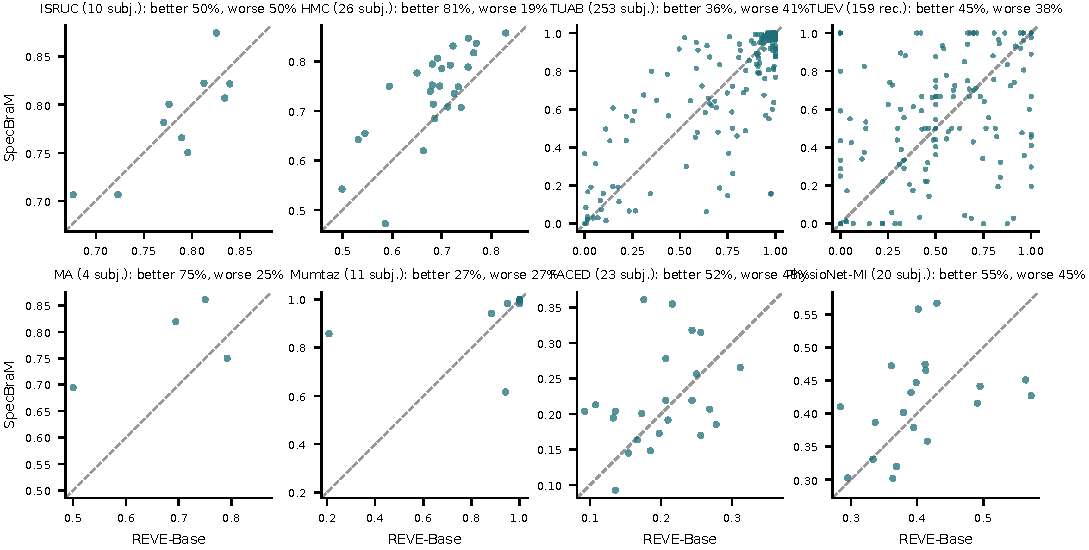
\includegraphics[width=\textwidth]{figures/per_subject.pdf}
\caption{\textbf{Per-subject balanced accuracy}, SpecBraM's main checkpoint vs.\ REVE-Base
(strict linear probe; one point per test subject, TUEV: per recording; dashed: equality).
Titles: share of subjects on which SpecBraM is better / worse.}
\label{fig:per_subject}
\end{figure*}
% auto-generated by make_case_figs.py -- do not edit
\begin{table}[h]\centering\small
\setlength{\tabcolsep}{3pt}
\caption{\textbf{Per-subject comparison}: percentage of test subjects (TUEV: recordings) on
which SpecBraM's balanced accuracy is higher / equal / lower than that of each external model
(strict linear probe, one checkpoint per model).}
\label{tab:per_subject}
\resizebox{\columnwidth}{!}{%
\begin{tabular}{l ccccc}
\toprule
Dataset & CBraMod & LaBraM-Base & BIOT & CSBrain & REVE-Base \\
\midrule
ISRUC (10 subj.) & 100/0/0 & 90/0/10 & 90/0/10 & 100/0/0 & 50/0/50 \\
HMC (26 subj.) & 100/0/0 & 96/0/4 & 96/0/4 & 100/0/0 & 81/0/19 \\
TUAB (253 subj.) & 60/13/27 & 65/10/25 & -- & 62/11/27 & 36/23/41 \\
TUEV (159 rec.) & 50/17/33 & 50/19/31 & -- & 45/21/34 & 45/18/37 \\
MA (4 subj.) & 75/0/25 & 100/0/0 & -- & 100/0/0 & 75/0/25 \\
Mumtaz (11 subj.) & 45/36/19 & 64/27/9 & -- & 82/18/0 & 27/45/28 \\
FACED (23 subj.) & 78/0/22 & 83/0/17 & -- & 65/0/35 & 52/0/48 \\
PhysioNet-MI (20 subj.) & 85/0/15 & 95/0/5 & -- & 90/0/10 & 55/0/45 \\
\bottomrule
\end{tabular}}
\end{table}


\subsection{Sleep Staging: ISRUC}
ISRUC subgroup~I \cite{khalighi2016isruc} contains one overnight polysomnography of each of
100 adults with sleep complaints, scored by experts in 30-s epochs into five AASM stages (W, N1,
N2, N3, REM). We use the six mastoid-referenced EEG leads (F3-A2, C3-A2, O1-A2, F4-A1, C4-A1,
O2-A1; 200\,Hz), of which F3/F4 are missing in some recordings, and the subject split of CBraMod
and CSBrain (subjects 1--80/81--90/91--100; 71{,}936/9{,}438/8{,}813 epochs). A 30-s epoch is represented by
the mean of the features of its three 10-s windows.
% auto-generated by make_arxiv_tables.py -- do not edit
\begin{table}[h]\centering\small
\setlength{\tabcolsep}{3pt}
\caption{\textbf{Detailed results on ISRUC} (strict linear probe). One checkpoint
per model, with the 95\% confidence interval from 1{,}000 bootstrap resamples of the
10 test subjects. Below SpecBraM's main
checkpoint: mean${\pm}$std over its three pretraining seeds. Bold: best per column.}
\label{tab:det_isruc}
\resizebox{\columnwidth}{!}{%
\begin{tabular}{l ccc}
\toprule
Model & Balanced Acc. & Cohen's $\kappa$ & Weighted F1\\
\midrule
\textbf{SpecBraM} & \ci{0.790}{0.764}{0.816} & \ci{0.733}{0.692}{0.773} & \ci{\textbf{0.795}}{0.757}{0.830} \\
\quad{\footnotesize three seeds, mean${\pm}$std} & \val{0.797}{0.006} & \val{0.744}{0.010} & \val{0.803}{0.008} \\
CBraMod & \ci{0.728}{0.702}{0.752} & \ci{0.658}{0.608}{0.705} & \ci{0.734}{0.698}{0.770} \\
LaBraM-Base & \ci{0.752}{0.720}{0.777} & \ci{0.686}{0.642}{0.724} & \ci{0.754}{0.716}{0.787} \\
BIOT & \ci{0.736}{0.691}{0.771} & \ci{0.666}{0.601}{0.715} & \ci{0.740}{0.686}{0.785} \\
CSBrain & \ci{0.730}{0.706}{0.752} & \ci{0.674}{0.638}{0.714} & \ci{0.749}{0.719}{0.782} \\
REVE-Base & \ci{\textbf{0.793}}{0.765}{0.816} & \ci{\textbf{0.736}}{0.703}{0.769} & \ci{\textbf{0.795}}{0.765}{0.824} \\
\bottomrule
\end{tabular}}
\end{table}

\begin{figure}[h]\centering
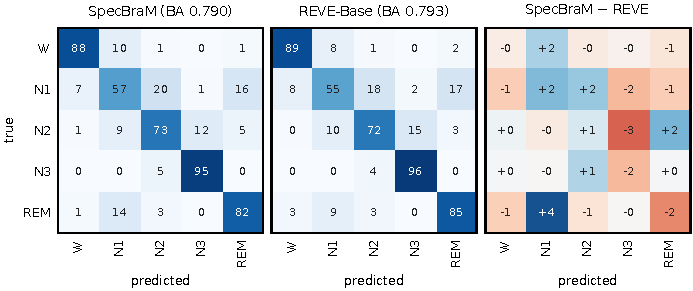
\includegraphics[width=\columnwidth]{figures/cm_isruc.pdf}
\caption{\textbf{Confusion matrices on ISRUC} (strict linear probe, row-normalized recall in \%): SpecBraM's main checkpoint, REVE-Base and their difference (blue: SpecBraM higher).}
\label{fig:cm_isruc}
\end{figure}
Fig.~\ref{fig:cm_isruc}: The two models make the same kinds of errors: N1 is confused with N2 and REM, and N3 with N2. Per-class recall differs by at most $2.4$ points, consistent with the small difference in balanced-accuracy point estimates.

\subsection{Sleep Staging: HMC}
HMC \cite{alvarez2021hmc} contains 151 clinical polysomnographies from the Haaglanden Medisch
Centrum, scored in 30-s epochs into the same five stages. We use the four EEG leads (F4-M1,
C4-M1, O2-M1, C3-M2; 256\,Hz) and the split of CBraMod and CSBrain by sorted subject ID
(100/25/26 recordings; 91{,}248/22{,}124/23{,}871 epochs). Epochs are represented as for ISRUC.
% auto-generated by make_arxiv_tables.py -- do not edit
\begin{table}[h]\centering\small
\setlength{\tabcolsep}{3pt}
\caption{\textbf{Detailed results on HMC} (strict linear probe). One checkpoint
per model, with the 95\% confidence interval from 1{,}000 bootstrap resamples of the
26 test subjects. Below SpecBraM's main
checkpoint: mean${\pm}$std over its three pretraining seeds. Bold: best per column.}
\label{tab:det_hmc}
\resizebox{\columnwidth}{!}{%
\begin{tabular}{l ccc}
\toprule
Model & Balanced Acc. & Cohen's $\kappa$ & Weighted F1\\
\midrule
\textbf{SpecBraM} & \ci{\textbf{0.742}}{0.699}{0.776} & \ci{\textbf{0.675}}{0.620}{0.724} & \ci{\textbf{0.751}}{0.707}{0.791} \\
\quad{\footnotesize three seeds, mean${\pm}$std} & \val{0.743}{0.002} & \val{0.675}{0.002} & \val{0.749}{0.003} \\
CBraMod & \ci{0.619}{0.576}{0.654} & \ci{0.513}{0.459}{0.567} & \ci{0.619}{0.572}{0.665} \\
LaBraM-Base & \ci{0.632}{0.583}{0.673} & \ci{0.530}{0.473}{0.585} & \ci{0.636}{0.586}{0.680} \\
BIOT & \ci{0.658}{0.609}{0.697} & \ci{0.562}{0.507}{0.615} & \ci{0.661}{0.616}{0.704} \\
CSBrain & \ci{0.611}{0.580}{0.641} & \ci{0.515}{0.472}{0.554} & \ci{0.625}{0.590}{0.660} \\
REVE-Base & \ci{0.704}{0.664}{0.737} & \ci{0.623}{0.577}{0.670} & \ci{0.707}{0.671}{0.745} \\
\bottomrule
\end{tabular}}
\end{table}

\begin{figure}[h]\centering
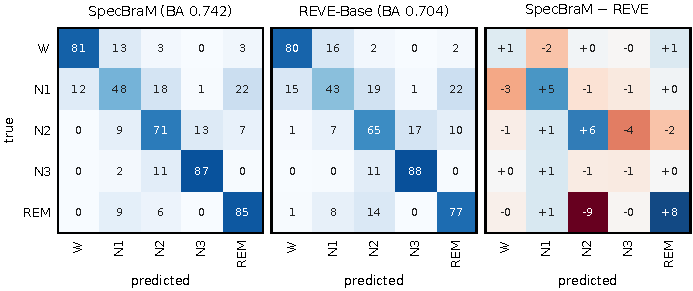
\includegraphics[width=\columnwidth]{figures/cm_hmc.pdf}
\caption{\textbf{Confusion matrices on HMC} (strict linear probe, row-normalized recall in \%): SpecBraM's main checkpoint, REVE-Base and their difference (blue: SpecBraM higher).}
\label{fig:cm_hmc}
\end{figure}
Fig.~\ref{fig:cm_hmc}: SpecBraM's lead over REVE comes from the transitional and REM stages: its recall is higher by $5.0$ points for N1, $6.0$ for N2 and $7.7$ for REM, while W and N3, the stages with the most distinct spectra, are recognized equally well by both.

\noindent\textbf{Case study: one night per dataset.} Fig.~\ref{fig:hypnogram} shows the
hypnograms of one test subject per sleep dataset, chosen by rule as the subject whose SpecBraM
balanced accuracy is closest to the median of its dataset, with the stages predicted by
SpecBraM, REVE and CBraMod from the frozen features of each 30-s epoch alone (no sequence
model). All models follow the sleep cycles; their errors concentrate at stage transitions and in
N1. On the ISRUC night the three models are close (balanced accuracy $0.800$, $0.776$ and $0.728$).
On the HMC night SpecBraM reaches $0.750$ against $0.594$ for REVE, which scores almost a third
of the N2 epochs as N3 (99 of 319 vs.\ 27 for SpecBraM) and half of the REM epochs as N2 (69 of
132 vs.\ 12), the same errors that dominate REVE's confusion matrix on the whole dataset
(Fig.~\ref{fig:cm_hmc}).
\begin{figure*}[t]\centering
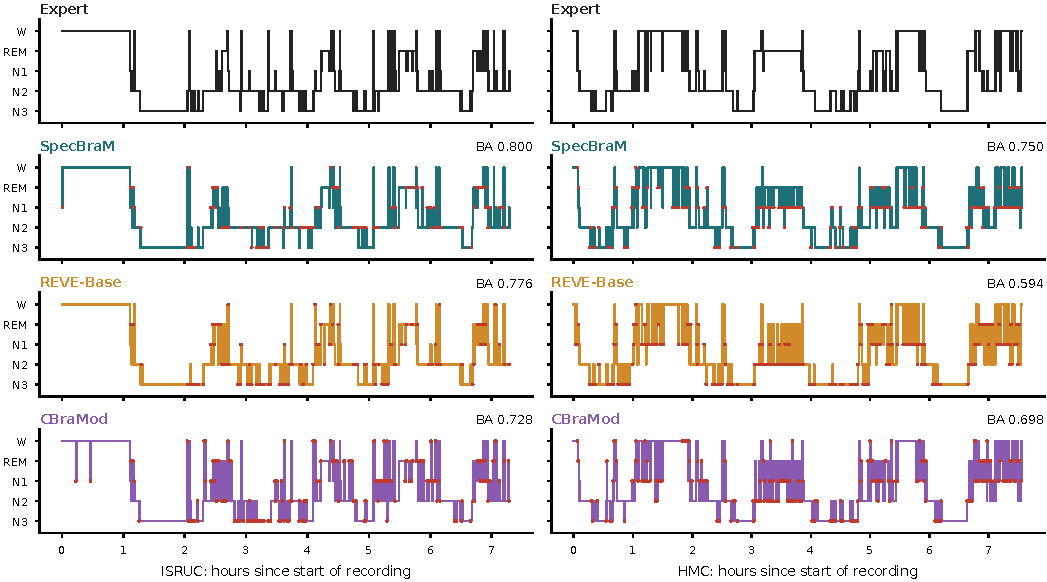
\includegraphics[width=\textwidth]{figures/hypnogram.pdf}
\caption{\textbf{Whole-night hypnograms} of one test subject per sleep dataset (left: ISRUC,
right: HMC; the subject whose SpecBraM balanced accuracy is closest to the dataset median).
Top: expert scoring; below: stages predicted by the strict linear probe on each model's frozen
features, epoch by epoch. Red dots: errors.}
\label{fig:hypnogram}
\end{figure*}

\subsection{Abnormal EEG Detection: TUAB}
TUAB \cite{obeid2016tuh} contains clinical EEG recordings of the Temple University Hospital
labeled normal or abnormal by neurologists. Following CBraMod, recordings are resampled to
200\,Hz, filtered (0.3--75\,Hz, 60\,Hz notch), converted to 16 bipolar channels of the TCP
montage and cut into non-overlapping 10-s windows that inherit the recording label. The official
evaluation folder is the test set; the training folder is split 80/20 by sorted patient ID
within each class (297{,}103/75{,}407/36{,}945 windows). The prepared metadata show three patients shared
between training and validation under this original per-class split. Test patients are disjoint
from both training and validation. All models use these same samples and splits; the overlap
limits validation independence. This downstream split issue is separate from possible TUEG
pretraining overlap.
% auto-generated by make_arxiv_tables.py -- do not edit
\begin{table*}[t]\centering\small
\setlength{\tabcolsep}{8pt}
\caption{\textbf{Detailed results on TUAB} (strict linear probe). One checkpoint
per model, with the 95\% confidence interval from 1{,}000 bootstrap resamples of the
253 test subjects. Below SpecBraM's main
checkpoint: mean${\pm}$std over its three pretraining seeds. Bold: best per column.}
\label{tab:det_tuab}

\begin{tabular}{l ccccc}
\toprule
Model & Balanced Acc. & Cohen's $\kappa$ & Weighted F1 & AUROC & AUC-PR\\
\midrule
\textbf{SpecBraM} & \ci{0.813}{0.775}{0.850} & \ci{0.627}{0.554}{0.700} & \ci{0.815}{0.778}{0.851} & \ci{\textbf{0.891}}{0.851}{0.924} & \ci{0.897}{0.860}{0.929} \\
\quad{\footnotesize three seeds, mean${\pm}$std} & \val{0.805}{0.007} & \val{0.611}{0.014} & \val{0.807}{0.007} & \val{0.880}{0.011} & \val{0.890}{0.008} \\
CBraMod & \ci{0.778}{0.738}{0.814} & \ci{0.558}{0.480}{0.629} & \ci{0.780}{0.742}{0.816} & \ci{0.856}{0.810}{0.894} & \ci{0.857}{0.812}{0.893} \\
LaBraM-Base & \ci{0.776}{0.740}{0.812} & \ci{0.554}{0.484}{0.624} & \ci{0.779}{0.744}{0.814} & \ci{0.856}{0.817}{0.891} & \ci{0.851}{0.806}{0.889} \\
CSBrain & \ci{0.772}{0.736}{0.805} & \ci{0.546}{0.475}{0.611} & \ci{0.774}{0.740}{0.807} & \ci{0.845}{0.804}{0.882} & \ci{0.836}{0.786}{0.878} \\
REVE-Base & \ci{\textbf{0.821}}{0.781}{0.861} & \ci{\textbf{0.644}}{0.565}{0.722} & \ci{\textbf{0.823}}{0.784}{0.861} & \ci{0.889}{0.848}{0.925} & \ci{\textbf{0.902}}{0.864}{0.933} \\
\bottomrule
\end{tabular}
\end{table*}

\begin{figure}[h]\centering
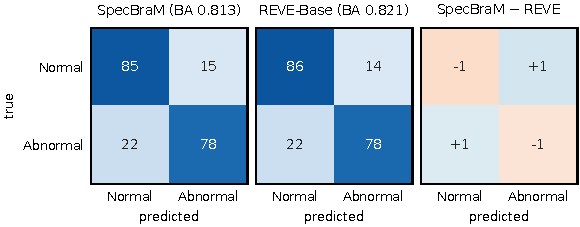
\includegraphics[width=\columnwidth]{figures/cm_tuab.pdf}
\caption{\textbf{Confusion matrices on TUAB} (strict linear probe, row-normalized recall in \%): SpecBraM's main checkpoint, REVE-Base and their difference (blue: SpecBraM higher).}
\label{fig:cm_tuab}
\end{figure}
Fig.~\ref{fig:cm_tuab}: Both models recognize normal and abnormal recordings almost equally well (recall within one point of each other); REVE's slightly higher balanced accuracy is spread over both classes.

\subsection{Event Classification: TUEV}
TUEV \cite{obeid2016tuh} annotates clinical EEG with six event classes: spike and sharp wave
(SPSW), generalized and lateralized periodic epileptiform discharges (GPED, PLED), eye movement
(EYEM), artifact (ARTF) and background (BCKG). Following CBraMod, each annotated 1-s event is
represented by a 5-s window centred on it, with the same filtering and 16-channel bipolar
montage as TUAB. The official evaluation folder is the test set and the training folder is split
80/20 by sorted patient ID (68{,}445/15{,}487/29{,}421 windows), with no patient overlap among the three
downstream splits. Background makes up 65\% of the windows; Cohen's
$\kappa$ and weighted F1 are dominated by it, whereas balanced accuracy weights the rare
epileptiform classes equally. This explains why REVE has the highest $\kappa$ and weighted F1
here although its balanced accuracy is below SpecBraM's and CSBrain's.
% auto-generated by make_arxiv_tables.py -- do not edit
\begin{table}[h]\centering\small
\setlength{\tabcolsep}{3pt}
\caption{\textbf{Detailed results on TUEV} (strict linear probe). One checkpoint
per model, with the 95\% confidence interval from 1{,}000 bootstrap resamples of the
159 test recordings. Below SpecBraM's main
checkpoint: mean${\pm}$std over its three pretraining seeds. Bold: best per column.}
\label{tab:det_tuev}
\resizebox{\columnwidth}{!}{%
\begin{tabular}{l ccc}
\toprule
Model & Balanced Acc. & Cohen's $\kappa$ & Weighted F1\\
\midrule
\textbf{SpecBraM} & \ci{0.555}{0.491}{0.648} & \ci{0.467}{0.369}{0.557} & \ci{0.722}{0.659}{0.777} \\
\quad{\footnotesize three seeds, mean${\pm}$std} & \val{0.561}{0.025} & \val{0.474}{0.049} & \val{0.724}{0.027} \\
CBraMod & \ci{0.525}{0.471}{0.609} & \ci{0.399}{0.327}{0.480} & \ci{0.669}{0.598}{0.742} \\
LaBraM-Base & \ci{0.468}{0.416}{0.545} & \ci{0.327}{0.228}{0.423} & \ci{0.624}{0.518}{0.710} \\
CSBrain & \ci{\textbf{0.564}}{0.505}{0.621} & \ci{0.421}{0.348}{0.489} & \ci{0.683}{0.619}{0.745} \\
REVE-Base & \ci{0.546}{0.500}{0.587} & \ci{\textbf{0.566}}{0.439}{0.655} & \ci{\textbf{0.778}}{0.727}{0.820} \\
\bottomrule
\end{tabular}}
\end{table}

\begin{figure}[h]\centering
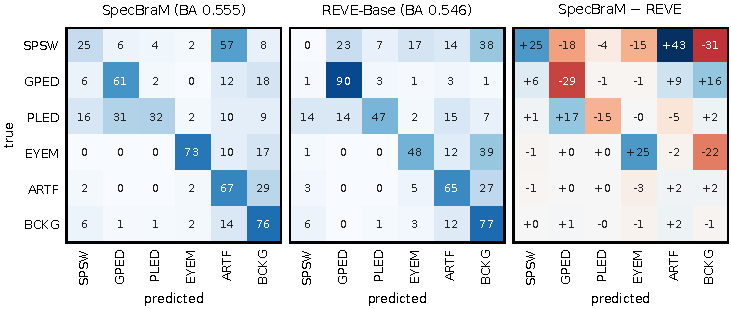
\includegraphics[width=\columnwidth]{figures/cm_tuev.pdf}
\caption{\textbf{Confusion matrices on TUEV} (strict linear probe, row-normalized recall in \%): SpecBraM's main checkpoint, REVE-Base and their difference (blue: SpecBraM higher).}
\label{fig:cm_tuev}
\end{figure}
Fig.~\ref{fig:cm_tuev}: The two models differ in kind. SpecBraM detects spike and sharp waves
(SPSW recall $25\%$ vs.\ $0\%$; REVE never predicts this class) and eye movements ($73\%$ vs.\
$48\%$), events with a distinct spectral signature. REVE is better on the periodic discharges
(GPED $90\%$ vs.\ $61\%$, PLED $47\%$ vs.\ $32\%$), which involve waveform shape and repetition
over seconds. This pattern is consistent with P4, but the models also differ in architecture
and pretraining data, so it does not isolate the effect of phase invariance.

\noindent\textbf{Examples.} Fig.~\ref{fig:tuev_cases} shows four test windows on which the two
models disagree, chosen by rule: for each class, the window that the correct model classifies
with the highest confidence. SpecBraM recognizes a spike and sharp wave that REVE labels as a
lateralized periodic discharge, and an eye-movement window that REVE labels as background. REVE
recognizes a generalized and a lateralized periodic discharge that SpecBraM labels as
background. In the GPED window the discharges recur about every two seconds across all
channels. Their waveform and repetition extend beyond the band power of a single 0.78-s patch.
The patch-local target does not directly supervise this longer temporal pattern (P4), although
the encoder can still represent temporal and waveform information.
\begin{figure*}[t]\centering
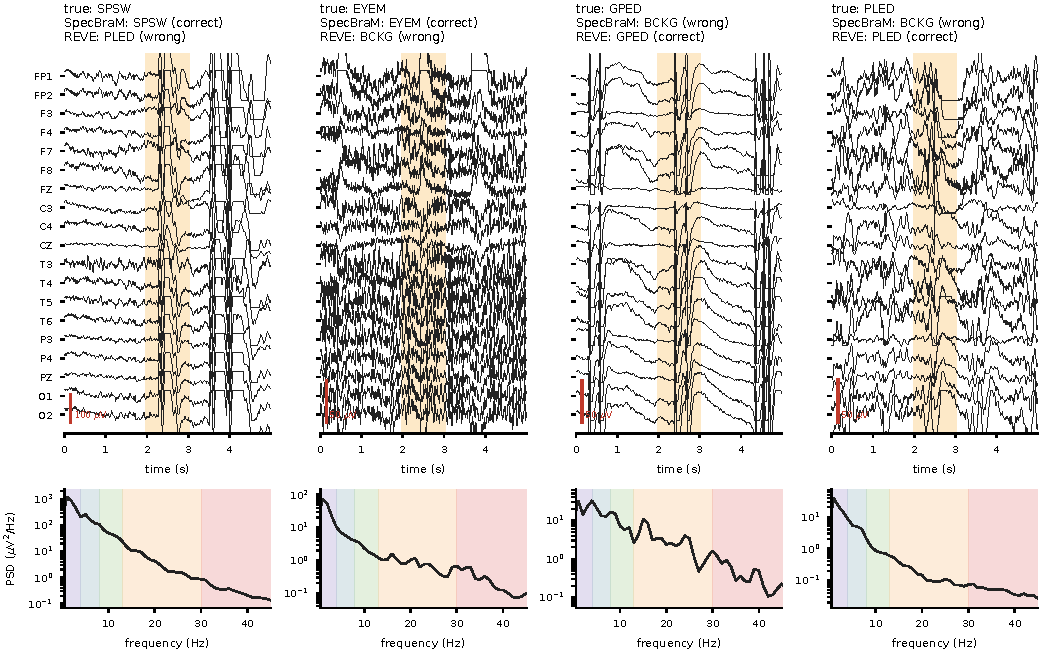
\includegraphics[width=\textwidth]{figures/tuev_cases.pdf}
\caption{\textbf{TUEV examples on which SpecBraM and REVE disagree} (strict linear probe; for
each class the window that the correct model classifies most confidently). Top: the 5-s window
(19 monopolar leads, CBraMod's preprocessing; shaded: the annotated 1-s event; traces clipped to
their row). Bottom: power spectral density averaged over channels, with the five bands of the
target.}
\label{fig:tuev_cases}
\end{figure*}

\subsection{Mental Workload: MA}
The mental arithmetic dataset \cite{zyma2019mentalarith} records 36 subjects at rest and during
serial subtraction with 20 leads (19 standard 10--20 leads and A2-A1; 500\,Hz). Following
CBraMod, recordings are resampled to 200\,Hz and cut into 5-s windows labeled rest or task, and
the sorted subjects are split 28/4/4 (1{,}343/172/192 windows). With four test subjects, MA has by far
the widest confidence intervals of all tasks.
% auto-generated by make_arxiv_tables.py -- do not edit
\begin{table*}[t]\centering\small
\setlength{\tabcolsep}{8pt}
\caption{\textbf{Detailed results on MA} (strict linear probe). One checkpoint
per model, with the 95\% confidence interval from 1{,}000 bootstrap resamples of the
4 test subjects. Below SpecBraM's main
checkpoint: mean${\pm}$std over its three pretraining seeds. Bold: best per column.}
\label{tab:det_ma}

\begin{tabular}{l ccccc}
\toprule
Model & Balanced Acc. & Cohen's $\kappa$ & Weighted F1 & AUROC & AUC-PR\\
\midrule
\textbf{SpecBraM} & \ci{\textbf{0.781}}{0.722}{0.840} & \ci{\textbf{0.583}}{0.526}{0.655} & \ci{\textbf{0.846}}{0.817}{0.876} & \ci{\textbf{0.912}}{0.878}{0.981} & \ci{\textbf{0.783}}{0.751}{0.942} \\
\quad{\footnotesize three seeds, mean${\pm}$std} & \val{0.747}{0.030} & \val{0.500}{0.093} & \val{0.810}{0.047} & \val{0.861}{0.052} & \val{0.706}{0.108} \\
CBraMod & \ci{0.653}{0.507}{0.799} & \ci{0.256}{0.011}{0.510} & \ci{0.686}{0.525}{0.811} & \ci{0.708}{0.532}{0.884} & \ci{0.515}{0.305}{0.730} \\
LaBraM-Base & \ci{0.681}{0.597}{0.736} & \ci{0.342}{0.205}{0.452} & \ci{0.746}{0.700}{0.793} & \ci{0.734}{0.649}{0.834} & \ci{0.571}{0.432}{0.724} \\
CSBrain & \ci{0.556}{0.403}{0.653} & \ci{0.095}{-0.175}{0.275} & \ci{0.626}{0.543}{0.711} & \ci{0.586}{0.402}{0.747} & \ci{0.306}{0.218}{0.451} \\
REVE-Base & \ci{0.684}{0.562}{0.771} & \ci{0.361}{0.143}{0.551} & \ci{0.758}{0.679}{0.838} & \ci{0.757}{0.669}{0.924} & \ci{0.587}{0.485}{0.802} \\
\bottomrule
\end{tabular}
\end{table*}

\begin{figure}[h]\centering
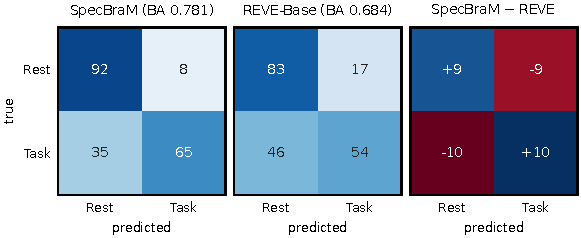
\includegraphics[width=\columnwidth]{figures/cm_ma.pdf}
\caption{\textbf{Confusion matrices on MA} (strict linear probe, row-normalized recall in \%): SpecBraM's main checkpoint, REVE-Base and their difference (blue: SpecBraM higher).}
\label{fig:cm_ma}
\end{figure}
Fig.~\ref{fig:cm_ma}: SpecBraM is better on both conditions (rest $+9.0$, task $+10.4$ points recall), so its lead is not a shift of the decision threshold.

\subsection{Depression: Mumtaz}
Mumtaz \cite{mumtaz2016mdd} contains resting-state EEG (eyes open and closed) of patients with
major depressive disorder and healthy controls, recorded with 19 linked-ear-referenced leads at
256\,Hz. Following CBraMod, recordings are resampled to 200\,Hz, filtered (0.3--75\,Hz, 50\,Hz
notch) and cut into 5-s windows that inherit the subject's diagnosis; recordings are split by
subject within each group (4{,}891/1{,}041/1{,}211 windows).
% auto-generated by make_arxiv_tables.py -- do not edit
\begin{table*}[t]\centering\small
\setlength{\tabcolsep}{8pt}
\caption{\textbf{Detailed results on Mumtaz} (strict linear probe). One checkpoint
per model, with the 95\% confidence interval from 1{,}000 bootstrap resamples of the
11 test subjects. Below SpecBraM's main
checkpoint: mean${\pm}$std over its three pretraining seeds. Bold: best per column.}
\label{tab:det_mumtaz}

\begin{tabular}{l ccccc}
\toprule
Model & Balanced Acc. & Cohen's $\kappa$ & Weighted F1 & AUROC & AUC-PR\\
\midrule
\textbf{SpecBraM} & \ci{\textbf{0.939}}{0.868}{0.995} & \ci{\textbf{0.879}}{0.733}{0.991} & \ci{\textbf{0.940}}{0.865}{0.995} & \ci{\textbf{0.991}}{0.964}{1.000} & \ci{\textbf{0.991}}{0.967}{1.000} \\
\quad{\footnotesize three seeds, mean${\pm}$std} & \val{0.942}{0.007} & \val{0.884}{0.015} & \val{0.942}{0.007} & \val{0.994}{0.003} & \val{0.994}{0.003} \\
CBraMod & \ci{0.893}{0.760}{0.988} & \ci{0.787}{0.513}{0.978} & \ci{0.893}{0.744}{0.989} & \ci{0.973}{0.911}{1.000} & \ci{0.973}{0.908}{1.000} \\
LaBraM-Base & \ci{0.876}{0.744}{0.986} & \ci{0.754}{0.484}{0.974} & \ci{0.877}{0.735}{0.987} & \ci{0.963}{0.882}{0.999} & \ci{0.960}{0.874}{0.999} \\
CSBrain & \ci{0.864}{0.774}{0.943} & \ci{0.727}{0.549}{0.887} & \ci{0.864}{0.772}{0.944} & \ci{0.947}{0.878}{0.990} & \ci{0.942}{0.862}{0.987} \\
REVE-Base & \ci{0.902}{0.743}{0.994} & \ci{0.804}{0.481}{0.989} & \ci{0.901}{0.728}{0.995} & \ci{0.968}{0.879}{1.000} & \ci{0.963}{0.861}{1.000} \\
\bottomrule
\end{tabular}
\end{table*}

\begin{figure}[h]\centering
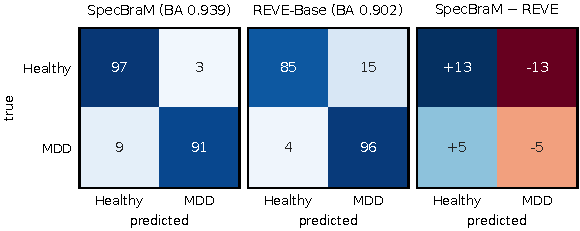
\includegraphics[width=\columnwidth]{figures/cm_mumtaz.pdf}
\caption{\textbf{Confusion matrices on Mumtaz} (strict linear probe, row-normalized recall in \%): SpecBraM's main checkpoint, REVE-Base and their difference (blue: SpecBraM higher).}
\label{fig:cm_mumtaz}
\end{figure}
Fig.~\ref{fig:cm_mumtaz}: SpecBraM's gain comes from fewer healthy subjects classified as depressed (recall of the healthy class $+12.6$ points), at a cost of $5.2$ points on the depressed class.

\subsection{Emotion Recognition: FACED}
FACED \cite{chen2023faced} records 123 subjects watching 28 video clips that elicit nine emotion
categories (anger, disgust, fear, sadness, neutral, amusement, inspiration, joy, tenderness),
with 32 leads at 250\,Hz. The last 30\,s of each clip are resampled to 200\,Hz and cut into three
10-s windows labeled with the clip's category; the sorted subjects are split 80/20/23
(6{,}720/1{,}680/1{,}932 windows; chance level $1/9$).
% auto-generated by make_arxiv_tables.py -- do not edit
\begin{table}[h]\centering\small
\setlength{\tabcolsep}{3pt}
\caption{\textbf{Detailed results on FACED} (strict linear probe). One checkpoint
per model, with the 95\% confidence interval from 1{,}000 bootstrap resamples of the
23 test subjects. Below SpecBraM's main
checkpoint: mean${\pm}$std over its three pretraining seeds. Bold: best per column.}
\label{tab:det_faced}
\resizebox{\columnwidth}{!}{%
\begin{tabular}{l ccc}
\toprule
Model & Balanced Acc. & Cohen's $\kappa$ & Weighted F1\\
\midrule
\textbf{SpecBraM} & \ci{\textbf{0.221}}{0.195}{0.248} & \ci{\textbf{0.126}}{0.096}{0.155} & \ci{\textbf{0.219}}{0.193}{0.245} \\
\quad{\footnotesize three seeds, mean${\pm}$std} & \val{0.216}{0.013} & \val{0.119}{0.015} & \val{0.214}{0.010} \\
CBraMod & \ci{0.171}{0.156}{0.188} & \ci{0.069}{0.052}{0.087} & \ci{0.167}{0.151}{0.182} \\
LaBraM-Base & \ci{0.167}{0.152}{0.181} & \ci{0.064}{0.047}{0.079} & \ci{0.163}{0.144}{0.177} \\
CSBrain & \ci{0.179}{0.161}{0.199} & \ci{0.077}{0.057}{0.098} & \ci{0.171}{0.153}{0.189} \\
REVE-Base & \ci{0.200}{0.179}{0.225} & \ci{0.101}{0.076}{0.130} & \ci{0.200}{0.177}{0.224} \\
\bottomrule
\end{tabular}}
\end{table}

\begin{figure*}[t]\centering
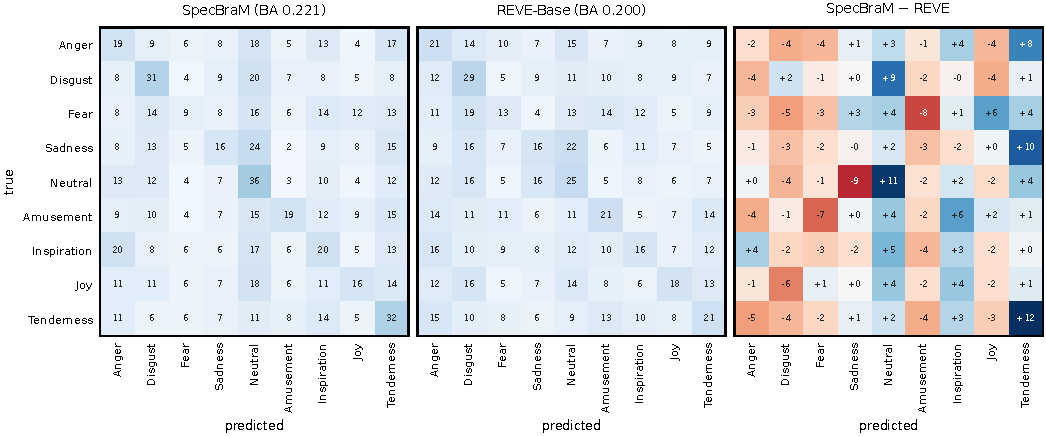
\includegraphics[width=\textwidth]{figures/cm_faced.pdf}
\caption{\textbf{Confusion matrices on FACED} (strict linear probe, row-normalized recall in \%): SpecBraM's main checkpoint, REVE-Base and their difference (blue: SpecBraM higher).}
\label{fig:cm_faced}
\end{figure*}
Fig.~\ref{fig:cm_faced}: Both models are far from perfect on nine emotions. SpecBraM's gain is concentrated on neutral ($+11.2$ points) and tenderness ($+11.6$), the two categories at the low-arousal end, while the other categories differ by a few points in either direction.

\subsection{Motor Imagery: PhysioNet-MI}
PhysioNet-MI \cite{schalk2004bci2000} records 109 subjects with 64 leads at 160\,Hz while they
imagine opening and closing the left fist, the right fist, both fists or both feet. Following
CBraMod, the imagery runs are high-pass filtered at 0.3\,Hz, notch filtered at 60\,Hz and
resampled to 200\,Hz, and the 4-s window after each cue is labeled with the imagined movement;
the sorted subjects are split 70/19/20 (6{,}300/1{,}734/1{,}803 windows; chance level $1/4$).
% auto-generated by make_arxiv_tables.py -- do not edit
\begin{table}[h]\centering\small
\setlength{\tabcolsep}{3pt}
\caption{\textbf{Detailed results on PhysioNet-MI} (strict linear probe). One checkpoint
per model, with the 95\% confidence interval from 1{,}000 bootstrap resamples of the
20 test subjects. Below SpecBraM's main
checkpoint: mean${\pm}$std over its three pretraining seeds. Bold: best per column.}
\label{tab:det_physio}
\resizebox{\columnwidth}{!}{%
\begin{tabular}{l ccc}
\toprule
Model & Balanced Acc. & Cohen's $\kappa$ & Weighted F1\\
\midrule
\textbf{SpecBraM} & \ci{\textbf{0.417}}{0.384}{0.450} & \ci{\textbf{0.223}}{0.179}{0.267} & \ci{\textbf{0.416}}{0.383}{0.449} \\
\quad{\footnotesize three seeds, mean${\pm}$std} & \val{0.397}{0.018} & \val{0.196}{0.024} & \val{0.396}{0.018} \\
CBraMod & \ci{0.312}{0.286}{0.340} & \ci{0.083}{0.048}{0.119} & \ci{0.310}{0.282}{0.337} \\
LaBraM-Base & \ci{0.299}{0.285}{0.314} & \ci{0.065}{0.047}{0.085} & \ci{0.299}{0.282}{0.312} \\
CSBrain & \ci{0.298}{0.273}{0.325} & \ci{0.064}{0.030}{0.100} & \ci{0.295}{0.270}{0.320} \\
REVE-Base & \ci{0.403}{0.371}{0.438} & \ci{0.204}{0.161}{0.250} & \ci{0.403}{0.371}{0.437} \\
\bottomrule
\end{tabular}}
\end{table}

\begin{figure}[h]\centering
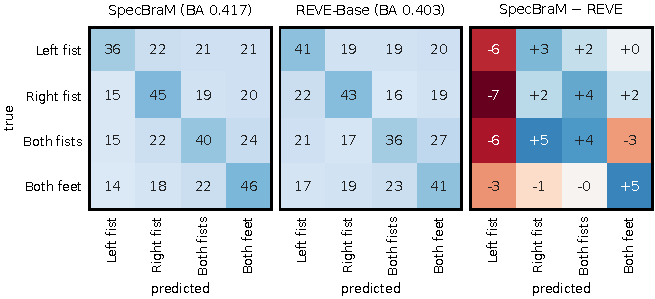
\includegraphics[width=\columnwidth]{figures/cm_physio.pdf}
\caption{\textbf{Confusion matrices on PhysioNet-MI} (strict linear probe, row-normalized recall in \%): SpecBraM's main checkpoint, REVE-Base and their difference (blue: SpecBraM higher).}
\label{fig:cm_physio}
\end{figure}
Fig.~\ref{fig:cm_physio}: SpecBraM is better on bilateral imagery (both fists $+4.2$, both feet $+4.9$ points) and slightly worse on the left fist ($-5.5$); distinguishing the left and right fist requires lateralized spatial patterns that a mean-pooled readout dilutes.


\section{Band Power versus Waveform Reconstruction beyond Sleep}\label{app:targettasks}
% auto-generated by make_arxiv_tables.py -- do not edit
\begin{table}[t]\centering\small
\setlength{\tabcolsep}{2.5pt}
\caption{\textbf{Band power vs.\ raw-waveform reconstruction beyond sleep} (same architecture,
data and steps; strict linear probe, balanced accuracy, mean${\pm}$std over three pretraining
seeds). Bold: best per column.}
\label{tab:target_tasks}
\resizebox{\columnwidth}{!}{%
\begin{tabular}{l cccccc}
\toprule
Target & TUAB & TUEV & MA & Mumtaz & FACED & PhysioNet-MI\\
\midrule
\textbf{Band power} (ours) & \val{\textbf{0.805}}{0.007} & \val{\textbf{0.561}}{0.025} & \val{\textbf{0.747}}{0.030} & \val{\textbf{0.942}}{0.007} & \val{0.216}{0.013} & \val{\textbf{0.397}}{0.018} \\
Raw-waveform reconstruction & \val{0.804}{0.002} & \val{0.533}{0.027} & \val{0.685}{0.051} & \val{0.924}{0.013} & \val{\textbf{0.220}}{0.010} & \val{0.395}{0.013} \\
\bottomrule
\end{tabular}}
\end{table}

Table~\ref{tab:target_tasks} extends the target study of Sec.~\ref{sec:targetstudy} to the other
tasks. Band power has higher mean scores on mental arithmetic ($+6.2$), depression screening
($+1.8$) and event classification ($+2.8$), and close mean scores on emotion recognition, motor
imagery and abnormality detection; these comparisons do not establish equivalence.

\section{Fine-Tuning}\label{app:fttasks}
% auto-generated by make_arxiv_tables.py -- do not edit
\begin{table*}[t]\centering\footnotesize
\setlength{\tabcolsep}{3pt}
\caption{\textbf{Sleep staging, fine-tuned} (5-class, 30-s epochs in sequences of 20, one
shared 1-layer sequence transformer; identical subject-disjoint splits as
\citet{csbrain}). Baselines as reported by \citet{csbrain} (REVE: its paper, ISRUC only).
Our rows: mean${\pm}$std over three \emph{pretraining} seeds (one fine-tuning run each), so
the spread includes pretraining variance, unlike the baselines' fine-tuning-seed spread.
Bold: best per column.}
\label{tab:ft30}
\resizebox{\textwidth}{!}{%
\begin{tabular}{l c ccc ccc}
\toprule
& & \multicolumn{3}{c}{ISRUC} & \multicolumn{3}{c}{HMC}\\
\cmidrule(lr){3-5}\cmidrule(lr){6-8}
Method & Pretrain (h) & BA & $\kappa$ & Weighted F1 & BA & $\kappa$ & Weighted F1\\
\midrule
\multicolumn{8}{l}{\emph{Task-specific models}}\\
EEGNet~\cite{lawhern2018eegnet} & -- & \val{0.7154}{0.0121} & \val{0.7040}{0.0173} & \val{0.7513}{0.0124} & \val{0.6534}{0.0122} & \val{0.5886}{0.0201} & \val{0.6536}{0.0168} \\
EEGConformer~\cite{song2023conformer} & -- & \val{0.7400}{0.0133} & \val{0.7143}{0.0162} & \val{0.7634}{0.0151} & \val{0.7149}{0.0086} & \val{0.6432}{0.0055} & \val{0.7080}{0.0039} \\
SPaRCNet~\cite{jing2023sparcnet} & -- & \val{0.7487}{0.0075} & \val{0.7097}{0.0132} & \val{0.7624}{0.0092} & \val{0.4756}{0.1109} & \val{0.3147}{0.1315} & \val{0.4108}{0.1310} \\
ContraWR~\cite{yang2023contrawr} & -- & \val{0.7402}{0.0126} & \val{0.7178}{0.0156} & \val{0.7610}{0.0137} & \val{0.4242}{0.0541} & \val{0.2340}{0.0554} & \val{0.2987}{0.0288} \\
CNN-Transformer~\cite{peh2022cnntransformer} & -- & \val{0.7363}{0.0087} & \val{0.7129}{0.0121} & \val{0.7719}{0.0153} & \val{0.6573}{0.0141} & \val{0.5961}{0.0105} & \val{0.6896}{0.0065} \\
FFCL~\cite{li2022ffcl} & -- & \val{0.7277}{0.0182} & \val{0.7016}{0.0292} & \val{0.7614}{0.0197} & \val{0.4427}{0.0702} & \val{0.2542}{0.0654} & \val{0.2902}{0.0485} \\
ST-Transformer~\cite{song2021sttransformer} & -- & \val{0.7381}{0.0205} & \val{0.7013}{0.0352} & \val{0.7681}{0.0175} & \val{0.2559}{0.0141} & \val{0.0503}{0.0183} & \val{0.1428}{0.0122} \\
\midrule
\multicolumn{8}{l}{\emph{Foundation models}}\\
BIOT~\cite{yang2023biot} & mixed & \val{0.7527}{0.0121} & \val{0.7291}{0.0230} & \val{0.7790}{0.0146} & \val{0.6862}{0.0041} & \val{0.6295}{0.0113} & \val{0.7091}{0.0147} \\
LaBraM-Base~\cite{jiang2024labram} & ${\sim}2.5$k & \val{0.7633}{0.0102} & \val{0.7231}{0.0182} & \val{0.7810}{0.0133} & \val{0.7277}{0.0101} & \val{0.6813}{0.0053} & \val{0.7454}{0.0027} \\
CBraMod~\cite{wang2025cbramod} & ${\sim}9$k & \val{0.7865}{0.0110} & \val{0.7442}{0.0152} & \val{0.8011}{0.0099} & \val{0.7269}{0.0041} & \val{0.6685}{0.0104} & \val{0.7395}{0.0089} \\
CSBrain~\cite{csbrain} & ${\sim}9$k & \val{0.7925}{0.0030} & \val{0.7406}{0.0102} & \val{0.7990}{0.0091} & \val{0.7345}{0.0047} & \val{0.6818}{0.0046} & \val{0.7506}{0.0042} \\
REVE~\cite{reve2025} & ${\sim}60$k & 0.7819 & 0.7500 & 0.8005 & -- & -- & -- \\
\midrule
Raw-waveform recon.\ (same arch.) & $2{,}388$ & \val{0.8062}{0.0061} & \val{0.7519}{0.0097} & \val{0.8100}{0.0069} & \val{0.7551}{0.0079} & \val{0.6935}{0.0057} & \val{0.7631}{0.0049} \\
\textbf{SpecBraM} & $2{,}388$ & \val{\textbf{0.8177}}{0.0032} & \val{\textbf{0.7670}}{0.0070} & \val{\textbf{0.8198}}{0.0051} & \val{\textbf{0.7696}}{0.0012} & \val{\textbf{0.7151}}{0.0021} & \val{\textbf{0.7796}}{0.0024} \\
\bottomrule
\end{tabular}}
\end{table*}

\noindent\textbf{Sleep staging.} Following CBraMod and CSBrain, 30-s epochs are grouped in
sequences of 20; each epoch is encoded (mean of its three 10-s windows), and a shared one-layer
transformer predicts one stage per epoch. Encoder and head are trained with AdamW (learning
rate $10^{-4}$, weight decay $0.05$) for up to 50 epochs with early stopping on validation
balanced accuracy (patience 10). SpecBraM reaches $0.8177{\pm}0.0032$ balanced accuracy on
ISRUC and $0.7696{\pm}0.0012$ on HMC (Table~\ref{tab:ft30}), above the listed published point estimates
(CSBrain $0.7925$/$0.7345$, REVE $0.7819$ on ISRUC), with the highest Cohen's $\kappa$ on both
datasets among the listed methods. The models differ in architecture, data and training recipe, and our standard
deviations are across pretraining seeds, unlike the baselines' fine-tuning seeds. After
fine-tuning, the gap to the matched raw-reconstruction model narrows to about $1.14$/$1.45$ points
($0.8062$/$0.7551$). In these sleep experiments, the target differences are larger for frozen
and low-label probes than after full fine-tuning.

% auto-generated by make_arxiv_tables.py -- do not edit
\begin{table}[t]\centering\small
\setlength{\tabcolsep}{2.5pt}
\caption{\textbf{Full fine-tuning beyond sleep} (balanced accuracy, mean${\pm}$std over three
pretraining seeds). Same samples and splits as the linear probe; encoder and a linear head on
mean-pooled tokens are trained with layer-wise learning-rate decay, and the epoch is selected on
validation balanced accuracy. Bold: best per column.}
\label{tab:ft_tasks}
\resizebox{\columnwidth}{!}{%
\begin{tabular}{l cccccc}
\toprule
Model & MA & Mumtaz & FACED & PhysioNet-MI & TUAB & TUEV\\
\midrule
\textbf{SpecBraM} & \val{\textbf{0.740}}{0.109} & \val{0.928}{0.026} & \val{\textbf{0.276}}{0.017} & \val{\textbf{0.564}}{0.027} & \val{\textbf{0.821}}{0.004} & \val{\textbf{0.650}}{0.079} \\
Raw-waveform recon.\ (same arch.) & \val{0.670}{0.018} & \val{\textbf{0.936}}{0.006} & \val{0.273}{0.013} & \val{0.531}{0.005} & \val{0.792}{0.006} & \val{0.566}{0.025} \\
\bottomrule
\end{tabular}}
\end{table}

\noindent\textbf{Other tasks.} Table~\ref{tab:ft_tasks} fine-tunes the encoder on the non-sleep
tasks, for SpecBraM and the matched raw-reconstruction model (layer-wise learning-rate decay,
early stopping on validation balanced accuracy). Band power has higher mean scores on mental
arithmetic, motor imagery, abnormality detection and event classification, and the mean scores
are close on depression screening and emotion recognition.

\section{Variants of the Band-Power Target}\label{app:variants}
% auto-generated by make_arxiv_tables.py -- do not edit
\begin{table*}[t]\centering\small
\setlength{\tabcolsep}{4pt}
\caption{\textbf{Spectral estimator of the band-power target} (linear patch embedding; everything else as
the main model). Strict linear probe on sleep staging, mean${\pm}$std over three pretraining
seeds unless stated; columns as Table~\ref{tab:ablation}. Bold: best per column.}
\label{tab:variants}
\begin{tabular}{l cc cc cc}
\toprule
& \multicolumn{2}{c}{BA (100\% labels)} & \multicolumn{2}{c}{BA (1\% labels)} & \multicolumn{2}{c}{$\Delta$ BA (pts)}\\
\cmidrule(lr){2-3}\cmidrule(lr){4-5}\cmidrule(lr){6-7}
Target & ISRUC & HMC & ISRUC & HMC & ISRUC & HMC\\
\midrule
\textbf{Band power} (main: periodogram, five classical bands) & \val{\textbf{0.7965}}{0.0059} & \val{0.7433}{0.0019} & \val{0.765}{0.006} & \val{0.670}{0.008} & -- & -- \\
\quad multitaper estimate (3 DPSS tapers, $NW{=}2$) & \val{0.7926}{0.0017} & \val{\textbf{0.7499}}{0.0064} & \val{\textbf{0.770}}{0.002} & \val{\textbf{0.686}}{0.005} & -0.4 & +0.7 \\
\bottomrule
\end{tabular}
\end{table*}

Table~\ref{tab:variants} varies the spectral estimator while keeping the main model otherwise
unchanged. With $0.78$-s patches the $\delta$ and $\theta$ bands contain only
three Fourier bins, motivating variance reduction (Table~\ref{tab:bins}). A multitaper estimate
(three DPSS tapers, $NW{=}2$) averages eigenspectra with ${\pm}2.6$\,Hz smoothing; the variance
reduction of the integrated log-band target is not measured here. It gives nearby full-label
mean scores and higher means with $1\%$ of the training epochs. Both estimators support strong
sleep representations, without identifying target-noise reduction as the cause.

\section{Factors besides the Target}\label{app:confounds}
% auto-generated by make_arxiv_tables.py -- do not edit
\begin{table}[t]\centering\small
\setlength{\tabcolsep}{3pt}
\caption{\textbf{Factors besides the target in the comparison with external models} (strict
linear probe, balanced accuracy; our rows: mean${\pm}$std over pretraining seeds). Per-channel
readout: tokens averaged over time within each channel and concatenated; still a frozen encoder
and a logistic regression. Our normalization for CBraMod/LaBraM: per-recording median/IQR
scaling, rescaled to the dataset's typical amplitude.}
\label{tab:confounds}
\resizebox{\columnwidth}{!}{%
\begin{tabular}{l cc cc}
\toprule
& \multicolumn{2}{c}{ISRUC} & \multicolumn{2}{c}{HMC}\\
\cmidrule(lr){2-3}\cmidrule(lr){4-5}
Model & (a) & (b) & (a) & (b)\\
\midrule
\multicolumn{5}{l}{\emph{Readout: (a) mean over all tokens (main protocol), (b) per-channel means}}\\
\textbf{SpecBraM} & \val{0.7965}{0.0059} & \val{0.7957}{0.0033} & \val{0.7433}{0.0019} & \val{0.7504}{0.0019} \\
Raw-waveform recon. & \val{0.7701}{0.0076} & \val{0.7734}{0.0039} & \val{0.7153}{0.0028} & \val{0.7220}{0.0041} \\
CBraMod & 0.7278 & 0.7708 & 0.6190 & 0.6841 \\
LaBraM-Base & 0.7523 & 0.7644 & 0.6323 & 0.6950 \\
CSBrain & 0.7304 & 0.7654 & 0.6114 & 0.6517 \\
REVE-Base & 0.7928 & 0.7995 & 0.7040 & 0.7223 \\
\midrule
\multicolumn{5}{l}{\emph{Input: (a) the model's own convention, (b) our per-recording normalization}}\\
CBraMod & 0.7278 & 0.7413 & 0.6190 & 0.6732 \\
LaBraM-Base & 0.7523 & 0.7326 & 0.6323 & 0.6524 \\
\midrule
\multicolumn{5}{l}{\emph{Scale: (a) 51.3M parameters, (b) 4.2M parameters (CBraMod: 4.0M)}}\\
Band power & \val{0.7965}{0.0059} & \val{0.7882}{0.0053} & \val{0.7433}{0.0019} & \val{0.7284}{0.0040} \\
Raw-waveform recon. & \val{0.7701}{0.0076} & \val{0.7537}{0.0042} & \val{0.7153}{0.0028} & \val{0.6738}{0.0083} \\
\bottomrule
\end{tabular}}
\end{table}

The comparison with external models (Sec.~\ref{sec:lpfm}) also differs in model size, input
convention and readout. Table~\ref{tab:confounds} varies each in turn. \emph{Readout}: averaging
tokens within each channel and concatenating the channels, still followed by a logistic
regression, raises CBraMod by $4.3$/$6.5$ points and LaBraM by $1.2$/$6.3$, while SpecBraM is
unchanged on ISRUC and gains $0.7$ on HMC; mean pooling therefore under-reads these models, but
SpecBraM still leads them by $2.5$--$6.6$ points. REVE-Base reaches $0.7995$ on ISRUC with this
readout, close to SpecBraM's point estimate. \emph{Input}: normalizing CBraMod's and LaBraM's input per
recording, as for our model, helps CBraMod ($+1.4$/$+5.4$) and is mixed for LaBraM
($-2.0$/$+2.0$). \emph{Scale}: at CBraMod's size (4.2M parameters) our band-power model loses
only $0.8$/$1.5$ points and still exceeds CBraMod by $6.0$/$10.9$, while raw reconstruction
loses $1.6$/$4.2$ points. Model size thus explains little of the gap to CBraMod and LaBraM, and
the target matters more at small scale.

\section{Handcrafted Spectral Features}\label{app:handcrafted}
% auto-generated by make_arxiv_tables.py -- do not edit
\begin{table*}[t]\centering\small
\setlength{\tabcolsep}{3pt}
\caption{\textbf{Handcrafted spectral features under the same strict linear probe} (balanced
accuracy). Basic: log absolute and relative power in the five classical bands per channel.
Rich: 1-Hz log PSD (0.5--45\,Hz), relative power in six bands, Hjorth parameters, spectral
entropy, 95\% spectral edge, line length and kurtosis per channel. Features are computed on our
input of each window (sleep: averaged over the three 10-s windows of an epoch, as for every
encoder). Bold: best per column.}
\label{tab:handcrafted}
\resizebox{\textwidth}{!}{%
\begin{tabular}{l cc cc cccccc}
\toprule
& \multicolumn{2}{c}{Sleep, 100\%} & \multicolumn{2}{c}{Sleep, 1\%} & \multicolumn{6}{c}{Beyond sleep}\\
\cmidrule(lr){2-3}\cmidrule(lr){4-5}\cmidrule(lr){6-11}
Features & ISRUC & HMC & ISRUC & HMC & MA & Mumtaz & FACED & PhysioNet-MI & TUAB & TUEV\\
\midrule
\textbf{SpecBraM} & \val{\textbf{0.7965}}{0.0059} & \val{\textbf{0.7433}}{0.0019} & \val{\textbf{0.765}}{0.006} & \val{0.670}{0.008} & \val{\textbf{0.747}}{0.030} & \val{\textbf{0.942}}{0.007} & \val{0.216}{0.013} & \val{0.397}{0.018} & \val{\textbf{0.805}}{0.007} & \val{\textbf{0.561}}{0.025} \\
Raw-waveform recon.\ (same arch.) & \val{0.7701}{0.0076} & \val{0.7153}{0.0028} & \val{0.721}{0.017} & \val{0.617}{0.017} & \val{0.685}{0.051} & \val{0.924}{0.013} & \val{\textbf{0.220}}{0.010} & \val{0.395}{0.013} & \val{0.804}{0.002} & \val{0.533}{0.027} \\
\midrule
Handcrafted: 5-band log/relative power & 0.7418 & 0.6825 & 0.707 & 0.624 & 0.663 & 0.926 & 0.201 & 0.391 & 0.735 & 0.498 \\
Handcrafted: rich spectral set & 0.7636 & 0.7227 & 0.747 & \textbf{0.674} & 0.712 & 0.906 & 0.217 & \textbf{0.410} & 0.752 & 0.469 \\
\bottomrule
\end{tabular}}
\end{table*}

Since the target is a spectral feature, a natural question is what self-supervision adds over
computing spectral features directly. Table~\ref{tab:handcrafted} probes two handcrafted feature
sets with the same protocol. The rich set is a strong reference: on sleep staging it exceeds
CBraMod and LaBraM and the raw-reconstruction model on HMC, but SpecBraM exceeds it by
$3.3$/$2.1$ points with all labels; with $1\%$ of the labels the two are close
($0.765$/$0.670$ vs.\ $0.747$/$0.674$). Beyond sleep, SpecBraM is clearly ahead on depression
screening and the two clinical tasks and about level on emotion recognition and motor imagery.
The handcrafted probes select the lower edge of the shared grid $C\in\{0.01,0.1,1\}$, so a
wider grid might raise them slightly.
